
% Copyright 2020 by Robert Hildebrand
%This work is licensed under a
%Creative Commons Attribution-ShareAlike 4.0 International License (CC BY-SA 4.0)
%See http://creativecommons.org/licenses/by-sa/4.0/

%\documentclass[../open-optimization/open-optimization.tex]{subfiles}
%
%\begin{document}

\chapter{Mathematical Programming}

\todoChapter{ {\color{gray} 50\% complete. Goal 80\% completion date: August 20}\\ 
Notes: This chapter is meant to be an introduction to all the types of deterministic problems that we might discuss.  It should list many applications, have a number of pictures, and describe how and where these types of problems are used.  }

\todo[inline]{Add intro that explains the format of problems, i.e., what the complexity comment means in each problem and add pointer to section on computational complexity.}
\todo[inline]{
Add discussion of Optimization, Operations Research, and Mathematical Programming including background and applications.   
Also, give an introduction to the content in this book, what you will learn by working though the book, and why this book is interesting and different from other sources.}

\begin{outcome}
\begin{itemize}
\item Identify reasons for studying operations research
\item Define "Mathematical Programming"
\item Learn about different applications of the tools in this book
\item Explore the different types of optimization models and what types we will see in this book
\end{itemize}
\end{outcome}
\section{Why study operations research?}

\section{What is Mathematical Programming?}

\section{Applications}


\section{Types of Optimization problems}
We will state main general problem classes to be associated with in these notes.  These are Linear Programming (LP), Mixed-Integer Linear Programming (MILP), Non-Linear Programming (NLP), and Mixed-Integer Non-Linear Programming (MINLP).  


%\begin{center}
%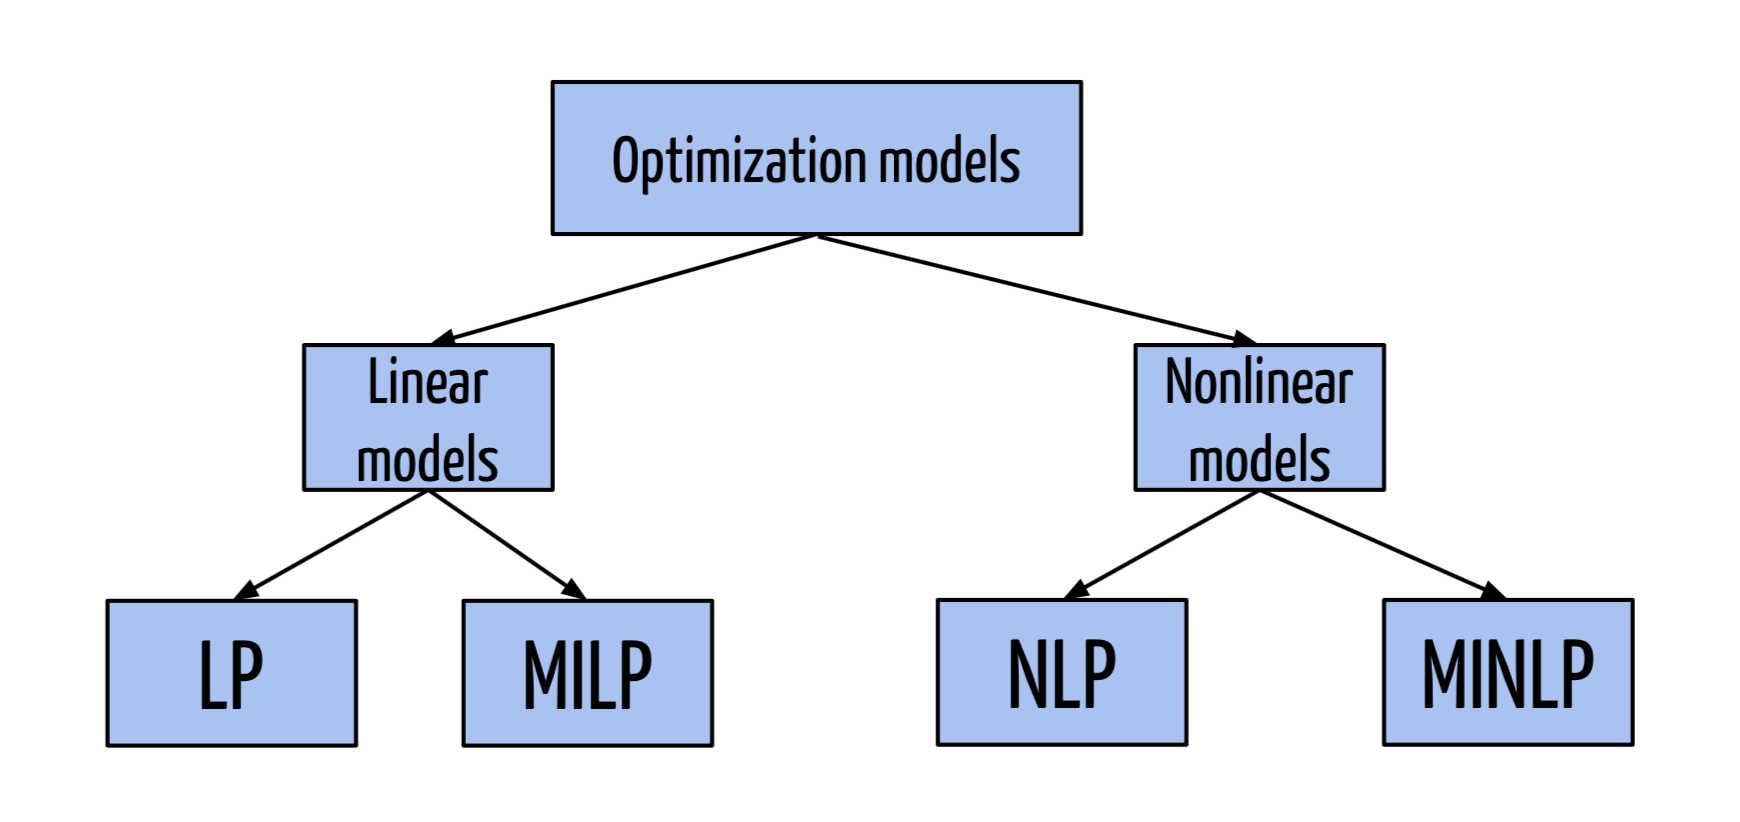
\includegraphics[scale = 0.5]{problem-class-diagram}\footnote{Diagram by Diego Moran}
%\end{center}

\includefigurestatic[][width = 1\linewidth][h]{problem-class-diagram}

Along with each problem class, we will associate a complexity class for the general version of the problem.  See \autoref{sec:complexity} for a discussion of complexity classes.  Although we will often state that input data for a problem comes from $\R$, when we discuss complexity of such a problem, we actually mean that the data is rational, i.e., from $\Q$, and is given in binary encoding.

\section{Linear Programming (LP)}
\todo[inline]{Describe applications and andd images}
Some linear programming background, theory, and examples will be provided in \autoref{sec:LP-background}.
\begin{general}{Linear Programming (LP)}{\polynomial}
%\label{general:LP}
Given a matrix $A \in \R^{m\times n}$, vector $b \in \R^m$ and vector $c \in \R^n$, the \emph{linear programming} problem is
\begin{equation}
\label{eq:LP}
\begin{split}
\max \quad & c^\top x\\
\st  \quad & Ax \leq b\\
& x \geq 0
\end{split}
\end{equation}
\end{general}

Linear programming can come in several forms, whether we are maximizing or minimizing, or if the constraints are $\leq, =$ or $\geq$.   One form commonly used is \emph{Standard Form} given as 
\begin{general}{Linear Programming (LP) Standard Form}{\polynomial}
Given a matrix $A \in \R^{m\times n}$, vector $b \in \R^m$ and vector $c \in \R^n$, the \emph{linear programming} problem in \emph{standard form} is
\begin{equation}
\label{eq:standardLP}
\begin{split}
\max \quad & c^\top x\\
\st  \quad & Ax = b\\
& x \geq 0
\end{split}
\end{equation}
\end{general}
\todo[inline]{Can shrink figure if there are not a lot of numbers of greek letters involved.}
\refincludefigurestatic[Linear programming constraints and objective.][scale = 0.2][h]{wiki/File/linear-programming.png}

\todo[inline]{Move this to simplex chapter}
\begin{exercise}
\label{exercise:LPconversion}
Start with a problem in form given as \eqref{eq:LP} and convert it to standard form \eqref{eq:standardLP} by adding at most $m$ many new variables and by enlarging the constraint matrix $A$ by at most $m$ new columns.
\end{exercise}
\section{Mixed-Integer Linear Programming (MILP)}
Mixed-integer linear programming will be the focus of Sections \ref{sec:IP-formulations},\ref{sec:exponential-IP-forumulations}, \ref{sec:IP-algorithms}, and \ref{sec:IP-heuristics}.
Recall that the notation $\Z$ means the set of integers and the set $\R$ means the set of real numbers.  The first problem of interest here is a \emph{binary integer program} (BIP) where all $n$ variables are binary (either 0 or 1).

\begin{general}{Binary Integer programming (BIP)}{\npcomplete}
Given a matrix $A \in \R^{m\times n}$, vector $b \in \R^m$ and vector $c \in \R^n$, the \emph{binary integer programming} problem is
\begin{equation}
\label{eq:BIP}
\begin{split}
\max \quad & c^\top x\\
\st  \quad & Ax \leq b\\
& x \in \{0,1\}^n
\end{split}
\end{equation}
\end{general}
A slightly more general class is the class of \emph{Integer Linear Programs} (ILP).  Often this is referred to as \emph{Integer Program} (IP), although this term could leave open the possibility of non-linear parts.

\refincludefigurestatic[Comparing the LP relaxation to the IP solutions.][scale = 0.3][h]{wiki/File/integer-programming.png}


\begin{general}{Integer Linear Programming (ILP)}{\npcomplete}
Given a matrix $A \in \R^{m\times n}$, vector $b \in \R^m$ and vector $c \in \R^n$, the \emph{integer linear programming} problem is
\begin{equation}
\label{eq:ILP}
\begin{split}
\max \quad & c^\top x\\
\st  \quad & Ax \leq b\\
& x \in \Z^n
\end{split}
\end{equation}
\end{general}


An even more general class is \emph{Mixed-Integer Linear Programming (MILP)}.  This is where we have $n$ integer variables $x_1, \dots, x_n \in \Z$ and $d$ continuous variables $x_{n+1}, \dots, x_{n+d} \in \R$.  Succinctly, we can write this as $x \in \Z^n \times \R^d$, where $\times$ stands for the \emph{cross-product} between two spaces.   

Below, the matrix $A$ now has $n+d$ columns, that is, $A \in \R^{m \times n+d}$.  Also note that we have not explicitly enforced non-negativity on the variables.  If there are non-negativity restrictions, this can be assumed to be a part of the inequality description $Ax \leq b$.
\begin{general}{Mixed-Integer Linear Programming (MILP)}{\npcomplete}
Given a matrix $A \in \R^{m\times (n+d)}$, vector $b \in \R^m$ and vector $c \in \R^{n+d}$, the \emph{mixed-integer linear programming} problem is
\begin{equation}
\label{eq:ILP}
\begin{split}
\max \quad & c^\top x\\
\st  \quad & Ax \leq b\\
& x \in \Z^n \times \R^d
\end{split}
\end{equation}
\end{general}

\section{Non-Linear Programming (NLP)}
\begin{general}{NLP}{\nphard}
Given a function $f(x)\colon \R^d \to \R$ and other functions $f_i(x)\colon \R^d \to \R$ for $i=1, \dots, m$,  the \emph{nonlinear programming} problem is
\begin{equation}
\label{eq:convex-programming}
\begin{split}
\min \quad & f(x)\\
\st  \quad & f_i(x) \leq 0  \quad  \text{ for } i=1, \dots, m\\
& x \in \R^d
\end{split}
\end{equation}
\end{general}


Nonlinear programming can be separated into convex programming and non-convex programming.  These two are very different beasts and it is important to distinguish between the two.
\subsection{Convex Programming}
Here the functions are all \textbf{convex!}
\begin{general}{Convex Programming}{\polynomial\ \  (typically)}
Given a convex function $f(x)\colon \R^d \to \R$ and convex functions $f_i(x)\colon \R^d \to \R$ for $i=1, \dots, m$,  the \emph{convex programming} problem is
\begin{equation}
\label{eq:convex-programming}
\begin{split}
\min \quad & f(x)\\
\st  \quad & f_i(x) \leq 0  \quad  \text{ for } i=1, \dots, m\\
& x \in \R^d
\end{split}
\end{equation}
\end{general}

Observe that convex programming is a generalization of linear programming.  This can be seen by letting $f(x) = c^\top x$ and $f_i(x) = A_i x - b_i$.  

\subsection{Non-Convex Non-linear Programming}
\todo[inline]{Move this to later chapter on complexity of NLP}
When the function $f$ or functions $f_i$ are non-convex, this becomes a non-convex nonlinear programming problem.  There are a few complexity issues with this.

\paragraph{IP as NLP}
As seen above, quadratic constraints can be used to create a feasible region with discrete solutions.  For example 
$$
x(1-x) = 0
$$
has exactly two solutions: $x = 0, x=1$.  
Thus, quadratic constraints can be used to model binary constraints.
\begin{general}{Binary Integer programming (BIP) as a NLP}{\nphard}
Given a matrix $A \in \R^{m\times n}$, vector $b \in \R^m$ and vector $c \in \R^n$, the \emph{binary integer programming} problem is
\begin{equation}
\label{eq:BIP}
\begin{split}
\max \quad & c^\top x\\
\st  \quad & Ax \leq b\\
& \hcancel[1.5pt]{x \in \{0,1\}^n}\\
& x_i(1-x_i) = 0 \quad \text{ for } i=1, \dots, n
\end{split}
\end{equation}
\end{general}

Alternatively, consider the transformation where $x_i \in \{-1,1\}$.
$$
\begin{aligned}
\min & c^\top x \\
\text { s.t. } & A x \leq b \\
& x \in \{-1,1\}^n
\end{aligned}
$$
This can be reformulated with a single nonconvex constraint as
$$
\begin{array}{cl}
\min & c^\top x \\
\text { s.t. } & A x \leq b \\
& -1 \leq x_j \leq 1, \quad 1 \leq j \leq n, \\
& \|x\|^2\geq n .
\end{array}
$$


\subsection{Machine Learning}
\todo[inline]{Many machine learning problems fall into this catrgory.  Todo: describe applications, give references, etc.}

Machine learning problems are often cast as continuous optimization problems, which involve adjusting parameters to minimize or maximize a particular objective.  Frequently they are convex optimization problems, but many turn out to be nonconvex.  Here are two examples of how these problems arise at a glance.  We will see examples in greater detail later in the book.

\subsubsection*{Loss Function Minimization}

In supervised learning, this objective is typically a loss function \( L \) that quantifies the discrepancy between the predictions of a model and the true data labels. The aim is to adjust the parameters \( \theta \) of the model to minimize this loss. Mathematically, this can be represented as:
\begin{equation}
\min_{\theta} L(\theta) = \min_{\theta} \frac{1}{N} \sum_{i=1}^{N} l(y_i, f(x_i; \theta))
\end{equation}
where \( N \) is the number of data points, \( l \) is a per-data-point loss (e.g., squared error for regression or cross-entropy for classification), \( y_i \) is the true label for the i-th data point, and \( f(x_i; \theta) \) is the model's prediction for the i-th data point with parameters \( \theta \).

\subsubsection*{Clustering Formulation}

Clustering, on the other hand, seeks to group or partition data points such that data points in the same group are more similar to each other than those in other groups. One popular method is the k-means clustering algorithm. The objective of k-means is to partition the data into \( k \) clusters by minimizing the within-cluster sum of squares (WCSS). The mathematical formulation can be given as:
\begin{equation}
\min_{\mathbf{c}_1, \ldots, \mathbf{c}_k} \sum_{j=1}^{k} \sum_{x_i \in C_j} \left\| x_i - \mathbf{c}_j \right\|^2
\end{equation}
where \( C_j \) represents the j-th cluster and \( \mathbf{c}_j \) is the centroid of that cluster.

This encapsulation presents a glimpse into how ML problems are framed mathematically. In practice, numerous algorithms, constraints, and regularizations add complexity to these basic formulations.


%\section{Mixed-Integer Non-Linear Programming (MINLP)}
%\todo[inline]{Fill in this section with formulas and discuss applications.  Most notable applications are Electrical Grid problems and Pooling problems. Find applications at Optimization and Engineering \url{https://link.springer.com/journal/11081/volumes-and-issues/21-4}}
\section{Mixed Integer Non-Linear Programming (MINLP)}

\begin{general}{MINLP}{\nphard}
Mixed Integer Nonlinear Programming (MINLP) combines elements of integer programming and nonlinear programming. In MINLP, some or all of the decision variables are constrained to be integers, and the objective function or constraints are nonlinear. A general MINLP problem can be formulated as:
\begin{equation}
\label{eq:minlp}
\begin{split}
\min \quad & f(x, y)\\
\st  \quad & g_i(x, y) \leq 0  \quad  \text{ for } i=1, \dots, m\\
           & h_j(x, y) = 0    \quad  \text{ for } j=1, \dots, p\\
           & x \in \R^n, y \in \Z^k
\end{split}
\end{equation}
where $f$ is the objective function, $g_i$ and $h_j$ are constraint functions, $x$ is a vector of continuous variables, and $y$ is a vector of integer variables.
\end{general}

MINLP is particularly challenging due to the nonlinearity in the objective and/or constraints and the discrete nature of some decision variables. It finds applications in various fields such as industry for process optimization, computational geometry, and machine learning for hyperparameter tuning.

\subsection{Convex MINLP}
In the convex case, both the objective function and the constraints are convex functions. This subclass is easier to solve compared to its non-convex counterpart.
\begin{general}{Convex MINLP}{\nphard, but \polynomial\ in fixed dimension\  (typically)}
For a convex MINLP, the problem is defined as:
\begin{equation}
\label{eq:convex-minlp}
\begin{split}
\min \quad & f(x, y) \quad \text{(convex)}\\
\st  \quad & g_i(x, y) \leq 0  \quad  \text{(convex constraints)}\\
           & x \in \R^n, y \in \Z^k
\end{split}
\end{equation}
\end{general}
Convex MINLPs, while still challenging, are typically more tractable due to the properties of convexity, which allow for more efficient solution methods.

\subsection{Non-Convex MINLP}
Non-convex MINLPs are significantly harder due to the presence of non-convex functions, which can lead to multiple local minima.
\begin{general}{Non-Convex MINLP}{\nphard (in fact, undecidable)}
The non-convex MINLP problem is formulated as:
\begin{equation}
\label{eq:nonconvex-minlp}
\begin{split}
\min \quad & f(x, y) \quad
\text{(non-convex)}\\
\st \quad & g_i(x, y) \leq 0 \quad \text{(possibly non-convex constraints)}\\
& x \in \R^n, y \in \Z^k
\end{split}
\end{equation}
\end{general}
Non-convex MINLPs pose significant computational challenges due to the possibility of multiple local optima and the inherent complexity of integer constraints. These problems are common in real-world applications where decisions are discrete, and the system behavior is non-linear and complex.

\subsection*{Complexity and Applications}
MINLP problems are known for their computational complexity, primarily due to the combination of non-linearity and integrality. The non-convex variants, in particular, are \nphard, making them some of the most challenging problems in optimization.

In practice, MINLP models find extensive applications across various domains. In industry, they are used for complex decision-making processes like supply chain optimization and production planning. In computational geometry, MINLP techniques help in solving problems like optimal packing or layout design. Furthermore, in the realm of machine learning, MINLPs are crucial for tasks like feature selection and hyperparameter optimization where discrete choices and nonlinear relationships are involved.

The versatility of MINLP models, combined with their inherent complexity, makes them a fascinating and essential area of study in the field of optimization.



%
%
%\end{document}
